\documentclass{article}
\usepackage[utf8]{inputenc}
\usepackage[spanish]{babel}
\usepackage{graphicx}
\usepackage{amsfonts}

\begin{document}
%Portada
  \begin{figure}[t]
    \begin{center}
        
\includegraphics[width=0.2\textwidth]{ull.eps}
        \hspace{5.5cm}
		
\includegraphics[width=0.2\textwidth]{fmatesc.eps}
    \end{center}
  \end{figure}
  \title{Integración Del Trapecio}
  \author{Tiffany López Nicholson \\ Miriam Martín Jacinto \\ Sergio Vega García}
  \date{\today}
  \maketitle

  \begin{abstract}
    \begin{center}
       A continuación se presentará como se ha implementado con python un algoritmo capaz de resolver la integral definida $\int_{1}^{6} \frac{1}{1+e^x}$
    \end{center}
  \end{abstract}
  \pagebreak

%%%%%%%%%%%%%%%%%%%%%

  \tableofcontents
  \pagebreak
  
%%%%%%%%%%%%%%%%%%%%%
  
  \section{Motivaciones y objetivos}
    \subsection{Objetivo principal}
       Debido a que realizar la Regla del Trapecio manualmente es muy tedioso, y por ende, se pierde mucho tiempo, se ha decidido implementar un programa en python que realice la Regla del Trapecio para f(x)
    \subsection{Objetivo específico} 
       El algoritmo que se desarrollará a lo largo del proyecto será capaz de resolver la integración del trapecio para $ f(x) = \frac{1}{1 + e^{x}}$, x E [1, 6]. Esto significaría una mayor rapidez para la obtención de resultados, y mayor presición.
  \pagebreak

%%%%%%%%%%%%%%%%%%%%%

  \section{Fundamentos teóricos}
    La regla del trapecio es un método de integración numérica que se basa en aproximar el valor de la integral definida de $f(x)$ por el de la función lineal que pasa a través de ésta, formándose una figura: un trapecio. Para obtener esta aproximación, debemos calcular el área de los trapecios.
    
    \begin{figure}[h]
      \begin{center}
	\includegraphics[scale=0.5]{areadeltrapecio.eps}
	\caption{Ejemplo}
      \end{center}
    \end{figure}

      Para justificar este método, deberemos ''aproximar'' de una buena manera nuestra función $f(x)$. Esto lo haremos gracias a la \textit{interpolación polinomial}.

    \subsection{Interpolación polinomial.}
      La interpolación polinomial nos dice que para hacer una ''buena aproximación''de $f(x)$, que querremos integrar, por otra función $g(x)$, en los puntos $x_{i}$ (con $i = 1, 2, 3, ..., n$); o lo que es lo mismo, $\int_{x_{1}}^{x_{n}}f(x)dx \approx \int_{x_{1}}^{x_{n}}g(x)dx$, $\forall x_{i}, con i = 1, 2, 3, ..., n$. Estas dos funciones deben ser continuas en el intervalo $[x_{1}, x_{n}]$.\\
      Pero el problema que se presenta es como buscar estas funciones. Hay varios teoremas que nos ayudan a resolverlo, como el \textit{teorema aproximación de Weierstrass}\footnote{http://es.wikipedia.org/wiki/Teorema\_de\_aproximación\_de\_Weierstrass} o el \textit{polinomio de interpolación de Lagrange}\footnote{http://es.wikipedia.org/wiki/Interpolación\_polinómica\_de\_Lagrange}.
      
    \subsection{Integración del trapecio}

      Para la utilización del método del trapecio partimos de una función, la cual dividiremos en n trozos iguales. Cuanto mayor sea el número de particiones, mayor precisión tendrá el método.\\

  	\begin{center}
         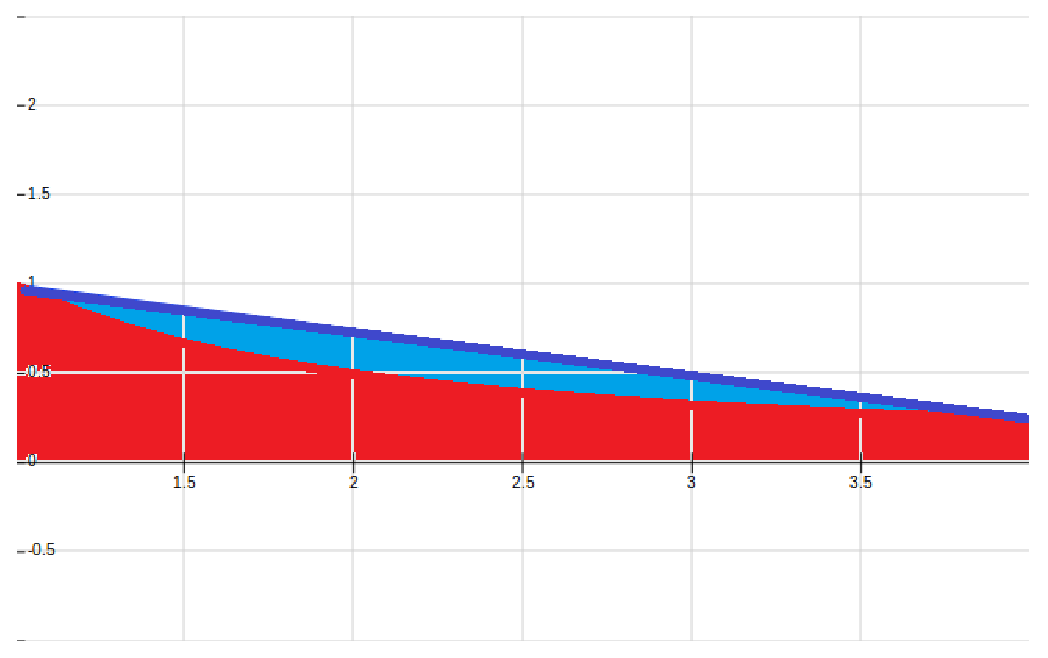
\includegraphics[width=0.48\textwidth]{img2.eps}
	 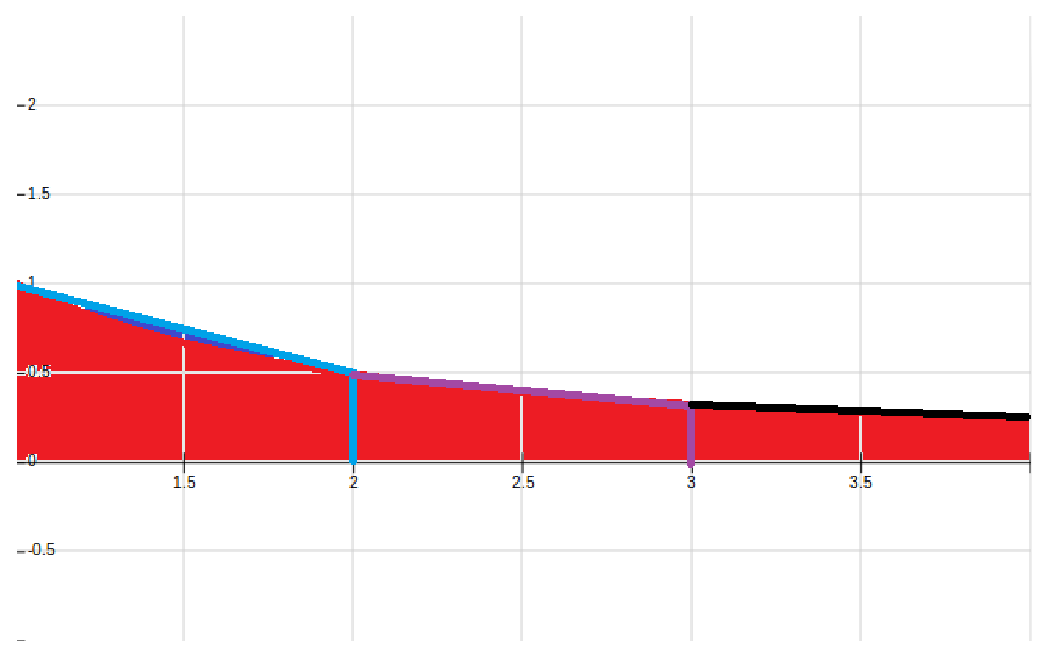
\includegraphics[width=0.48\textwidth]{img3.eps}
        \end{center}


      Se puede apreciar que el área tomada por exceso, es decir, la que supera a la función, o la tomada por defecto, la cual no llega a la función, se reduce según aumenta el número de particiones. \\
      \\

      La función general es: 
        
      \begin{center}
   
        $\int_{a}^{b}f(x)dx \approx \frac{h}{2}[f(a)-2f(a+h)+2f(a+2h)+...+f(b)]$

      \end{center}
 
      Donde $h=\frac{b-a}{n}$ y n es el número de divisiones.\\

      La expresión anterior también se puede escribir como:

      \begin{center}

        $\int_{a}^{b}f(x)dx \approx \frac{b-a}{n}(\frac{f(a)+f(b)}{2}+\sum\limits_{k=1}^{n-1}f(a+k\frac{b-a}{n}))$
      \end{center}

    \subsection{Integración del trapecio aplicado}
      
    La ecuación específica del proyecto es $f(x)\frac{1}{1+e^x}$, cuya representación gráfica es la siguiente:
     
     \begin{figure}[h]
      \begin{center}
         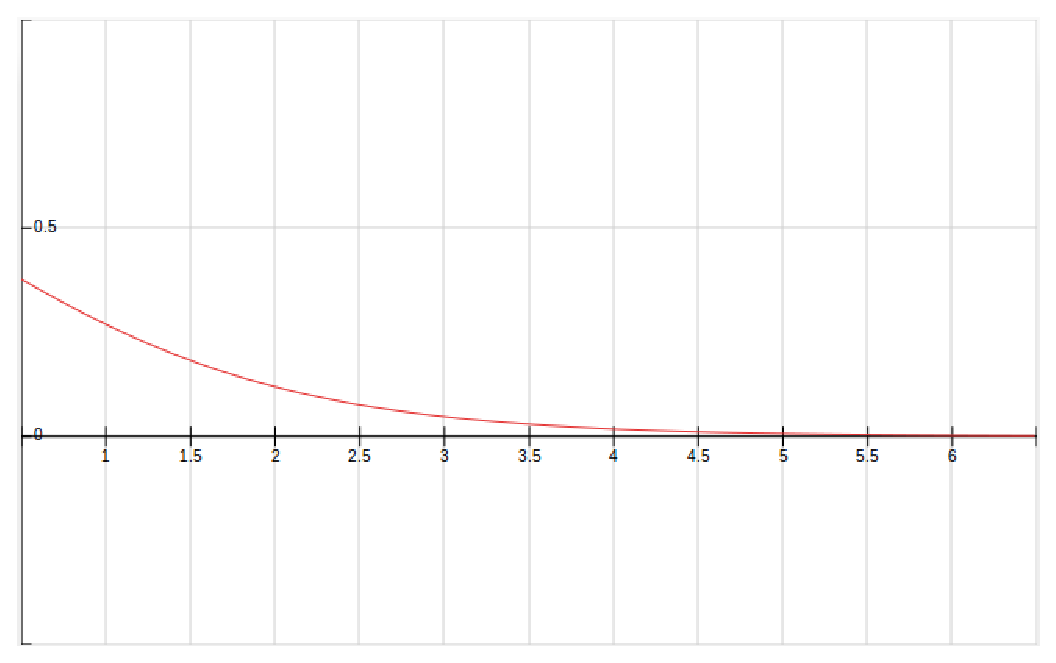
\includegraphics[width=0.7\textwidth]{img4.eps}\caption{Prueba}\label{fig:grafica}
      \end{center}
     \end{figure}

      El intervalo de la integral es [1,6]. Existe función en todos los puntos, por lo que también existe la integral. Al igual que en el caso anterior, por existir una curva, habría que realizar varias particiones para conseguir un resultado preciso.

   \pagebreak

%%%%%%%%%%%%%%%%%%%%%%%%%%%%%%%%%%

%BOCETOOOOOOOOOOOO

   \section{Procedimiento experimental}
   Para poder realizar la integración del trapecio primero necesitabamos analizar los datos iniciales.
   \begin{itemize}
    \item La función $f(x)=\frac{1}{1+e^x}$ estaba definida en el intervalo [1,6].
    \item La función definida en [1,6] existe en $\mathbb{R}$, numeros reales, por tanto se puede integrar.
    \item En la fórmula de la integración del trapecio intervienen bastantes variables.
   \end{itemize}
   Con estos datos a priori se pueden sacar dos conclusiones.
     \begin{enumerate}
       \item Realizar la integración por la regla del trapecio manualmente es muy tedioso.
       \item Se necesita implementar un programa en python para agilizar la tarea.
     \end{enumerate}

   Se ha creado en python un programa que permita elegir el número de particiones y así comparar resultados. La utilidad principal sería comprobar que cuantas más particiones se realicen, más precisa es la integración.
    
    \subsection{Descripción de los experimentos}

   Se ha implementado un programa en python capaz de realizar la regla del trapecio, y que podamos elegir particiones mínimas y máximas. Al ejecutarlo e introducir los datos nos va mostrando los resultados de cada partición.\\

   Se han comprobado algunas particiones manualmente para comprobar que realmente el programa está funcionando correctamente.\\

   Se ha ejecutado dos veces el bucle con las siguientes caracteristicas:
 
   \begin{enumerate}
     \item De 1 a 10 particiones, con intervalo de 1 unidad.
     \item De 10 a 100 particiones, con intervalo de 10 unidades.
     \item De 100 a 1000 particiones, con intervalo de 100 unidades.
   \end{enumerate}

    \subsection{Descripción de las computadoras utilizadas:}

      \begin{itemize}
        \item S.O.: Linux - Ubuntu
        \item Procesador: Pentium(R) Dual-Core CPU  T4400  @ 2.20GHz
        \item Velocidad: 1200.000 MHz
        \item RAM: 4 GB
        \item Versión de Python: 2.7.3
      \end{itemize}

    \subsection{Resultados obtenidos}

     \begin{tabular}{|c|c|c|c|}
      \hline
      Partición & Resultado & Partición & Resultado\\
      \hline
      1 & 0.6908982271 & 10 & 0.316070258216\\
      \hline
      2 & 0.418729690428 & 20 & 0.312415536652\\ 
      \hline
      3 & 0.360170903466 & 30 & 0.311647557367\\
      \hline
      4 & 0.339273533105 & 40 & 0.311347886591\\
      \hline
      5 & 0.329487501506 & 50 & 0.311195057792\\
      \hline
      6 & 0.324106360674 & 60 & 0.311104409514\\
      \hline
      7 & 0.320820024708 & 70 & 0.311045164508\\
      \hline
      8 & 0.31865911442 & 80 & 0.311003740508\\
      \hline
      9 & 0.317158073083 & 90 & 0.310973305356\\
      \hline
      10 & 0.316070258216 & 100 & 0.310950080829\\
      \hline
      Tiempo & 0.000426054000854 & Tiempo & 0.00157999992371\\ \hline
     \end{tabular}

     \vspace{0.4cm}
    \begin{center}
     \begin{tabular}{|c|c|}
      \hline
      Partición & Resultado\\
      \hline
      100 & 0.310950080829\\ 
      \hline
      200 & 0.310857929721\\ 
      \hline
      300 & 0.310831706878\\ 
      \hline
      400 & 0.310819438106\\
      \hline
      500 & 0.310812346491\\
      \hline
      600 & 0.310812346491\\
      \hline
      700 & 0.310804489423\\ 
      \hline
      800 & 0.310802088259\\
      \hline
      900 & 0.310800238521\\
	  \hline
      1000 & 0.310798769966\\ 
      \hline
      Tiempo & 0.0125889778137\\ \hline
     \end{tabular} 
    \end{center}
    \subsection{Análisis de resultados}

     Analizando los resultados, se observa que no hay grandes cambios a partir de la octava división. Si solo se hicieran una o dos divisiones se tendría un resultado mucho mayor del real, eso es porque hay una curva pronunciada, sobre todo al principio. Se puede apreciar en la Figura ~\ref{fig:grafica}. Si fuera una recta no habría variación en ninguna de las particiones.\\

     Cuanto mayor es el número de particiones, más se reduce el resultado, por tanto la curva que existe es decreciente.\\

     El número de particiones influye en el tiempo que tarda en obtenerse el resultado, incluso en un ordenador, pero es notorio cuando la cantidad de particiones es alta.\\

     % SACAR MÁS CONCLUSIONES

    \pagebreak

   \section{Conclusiones}
    El tipo de función determina la cantidad mínima de particiones para una buena aproximación de la función.\\

    El método del trapecio es muy útil cuando la integral es muy difícil, pero tiene el problema de lo largo que es el método. Sin embargo, mediante un programa en python es todo mucho más sencillo.\\

    Es mejor utilizar un programa sobre todo para realizar comparaciones entre varias particiones, ya que tendrías los resultados casi al instante.\\

    Por otro lado, si la ecuación se puede integrar relativamente fácil, no sería necesario estar realizando la regla del trapecio, sino es mejor usar directamente las igualdades notables.\\

   % MÁS CONCLUSIONES
   \pagebreak

   \section{Apéndice}
    \subsection{Algoritmo}
   NOMBRE: Trapecio.py\\
   
   AUTORES:

   \begin{itemize}
     \item Tiffany López Nicholson
     \item Miriam Martín Jacinto
     \item Sergio Vega García
   \end{itemize}

   FECHA: \today \\

   DESCRIPCIÓN:\\

     Se pide introducir por teclado la cantidad mínima de particiones, la cantidad máxima y la cantidad de intervalos.\\

     El primer bucle es el encargado de las particiones, y el segundo, del sumatorio presente en la fórmula. Se imprime por teclado el resultado, y continúa ejecutándose el primer while.\\
   

%FIN BOCETO
%%%%%%%%%%%%%%%%%%%%%%%%%%%%%%%%%%
\end{document}
